\section{Overview}
\label{sec: overview}%


\section{Component View}
\label{sec: component_view}%
The component diagram shows all the identified components.
It also describes the relations between the modules, representing the verse of the communication flow and the actors of it.
Before showing the diagram, there must be clarifications about it:
\begin{itemize}
    \item Two client applications are represented, one for both EVD and CPO. They are the same client application.
    We preferred to double the module in the diagram to facilitate comprehension of how users communicate with the system.
    \item For the same reasons, there are duplicated interfaces offered by components.
    \item The diagram shows a macro component called \verb|eMALL| that represents the whole system.
    Outside the system, they are shown the external services, the DBMSs, and the client application.
    Communication between modules and \verb|eMALL| happens thanks to interfaces that the system offers or exploits, depending on the component.
\end{itemize}
After the diagram, it will follow a brief description of each identified component.

\subsection{Component diagram}
\label{subsec:component_diagram}%
\begin{figure} [H]
    \begin{center}
        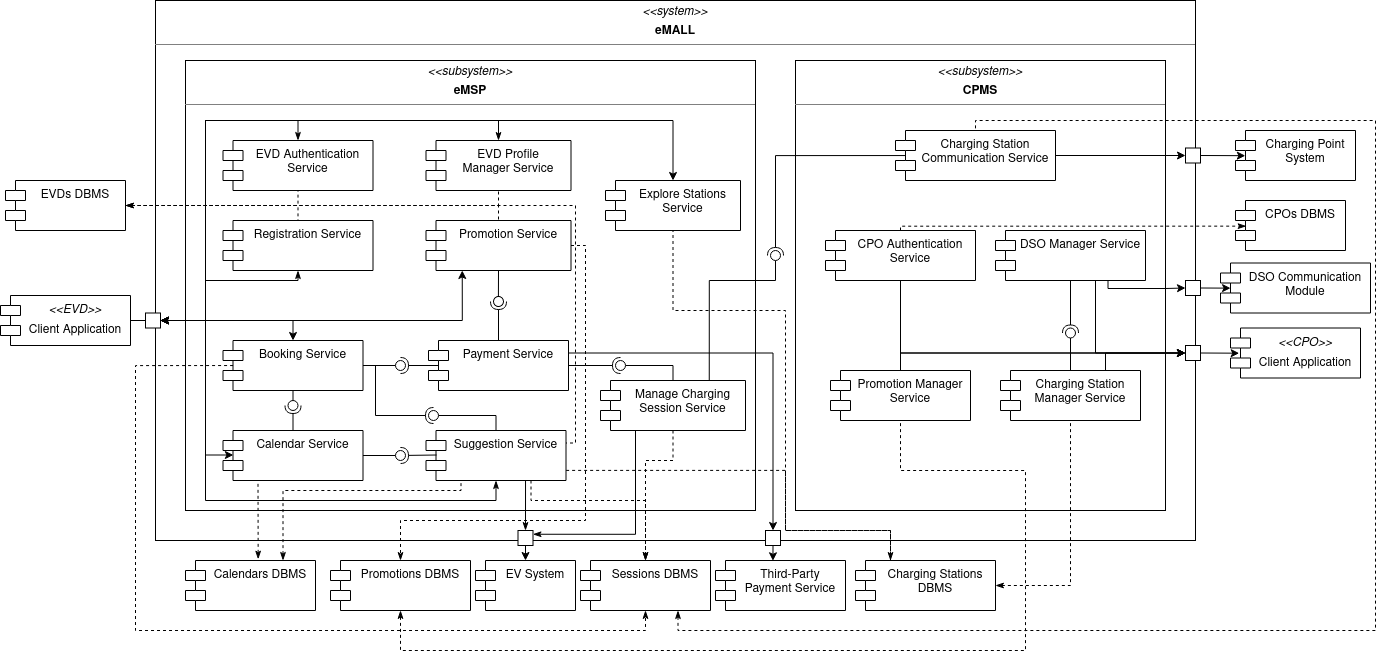
\includegraphics[width=1\linewidth]{ComponentDiagram/component_diagram}
        \caption{Component diagram of the eMALL system.}
        \label{fig: cd}
    \end{center}
\end{figure}

\subsection{Components description}
\label{subsec:components_description}%
The components are:
\begin{itemize}
    \item \textbf{Client Application.} \verb|Client Application| represent the client system used to connect and to communicate
    with \verb|eMALL|.
    \item \textbf{Registration Service.} \verb|Registration Service| handles the process of the creation
    of a new account requested by a new EVD user.
    It communicates with \verb|EVDs DBMS| to save the information about the new created account.
    \item \textbf{EVD Authentication Service.} \verb|EVD Authentication Service| handles the login process requested by an EVD\@.
    To do that, it communicates with \verb|EVDs DBMS| to validate the inserted credentials.
    \item \textbf{EVD Profile Manager Service.} \verb|EVD Profile Manager Service| offers the possibility to query
    the \verb|EVDs DBMS| in order to get requested information.
    In general, it is the service offered to the user to get or update information of the profile.
    So, he communicates with \verb|EVDs DBMS|.
    \item \textbf{Explore Stations Service.} \verb|Explore Stations Service| is the service used by the EVDs to navigate
    into the map of charging station that can be found around user's position.
    To do that, he needs stations position, so it communicates with \verb|Charging Stations DBMS|.
    Furthermore, it communicates also with the external service \verb|Navigator System|, used to elaborate positions
    and to show them into the map.
    \item \textbf{Booking Service.} \verb|Booking Service| is the module used to handle booking requests.
    It communicates with \verb|Sessions DBMS| to save the information about bookings and with \verb|Calendar Service|
    to start the process of insertion of a new activity into EVD's calendar representing the booked reservation.
    \item \textbf{Manage Charging Session Service.} \verb|Manage Charging Session Service| handles the charging session process.
    It allows the EVDs to start and interrupt the session and to pay for the service the user enjoyed.
    Furthermore, it sends to the EVDs notifications about ongoing session status.
    The module communicates with \verb|Charging Station Communication Service| to delegate the communication with the charging point
    where the EVD wants to charge the EV\@.
    As said before, the service offers the EVD the interface to make the payment of the session, so it communicates with
    \verb|Payment Service|.
    After the payment, the module saves the receipt of the session communicating the \verb|Sessions DBMS| module.
    \item \textbf{Promotion Service.} \verb|Promotion Service| offers the EVDs the possibility to activate special promotions
    activated by CPOs.
    To get the list of active promotions, it communicates with \verb|Promotions DBMS|.
    The module communicates also with \verb|EVD Profile Manager Service| to delegate the save of the activation of a special offer into
    the \verb|EVDs DBMS|.
    \item \textbf{Calendar Service.} \verb|Calendar Service| is module that manages EVDs calendar.
    It offers the possibility to visualize the calendar, saved events and their details.
    It also offers the functionality of activity insertion.
    To save all this information, the module communicates with \verb|Calendars DBMS|.
    After a new activity is inserted, \verb|Calendar Service| activates the process offered by \verb|Suggestion Service|
    in order to create suggestion about when and where the EVD should charge the EV\@.
    \item \textbf{Suggestion Service.} \verb|Suggestion Service| communicates with different modules to create suggestions.
    It communicates with:
    \begin{itemize}
        \item \verb|EVDs DBMS| to get user's EV specifications.
        \item \verb|Calendar DBMS| to get EVD's schedule to know precedent events that could affect the research.
        \item \verb|EV System| to get current EV status.
        \item \verb|Charging Stations DBMS| to get positions of the memorized charging stations.
        \item \verb|Navigation System| to calculate the path between the positions defined in the schedule of the EVD,
        and to identify which charging stations can be suggested to the user.
        \item \verb|Sessions DBMS| to get schedules of the charging point, getting in this way their available timeframes,
        and to see if there are other bookings done by the EVD\@.
        \item \verb|Booking Service| to start the booking process after the EVD confirms the received suggestion.
    \end{itemize}
    \item \textbf{Payment Service.} \verb|Payment Service| offers the possibility to pay for a service the EVD enjoyed.
    It communicates with \verb|EVD Profile Manager Service| to get EVD's payment methods.
    Once it has the needed information, it communicates with \verb|Third-Party Payment Service| to make the payment.
    \item \textbf{CPO Authentication Service.} \verb|CPO Authentication Service| handles the login process requested by a CPO\@.
    To do that, it communicates with \verb|CPOs DBMS| to validate the inserted credentials.
    \item \textbf{CPO Profile Manager Service.} \verb|CPO Profile Manager Service| offers the possibility to query
    the \verb|CPOs DBMS| in order to get requested information.
    In general, it is the service offered to the user to get or update information of the profile.
    So, he communicates with \verb|CPOs DBMS|.
    \item \textbf{Charging Station Manager Service.} \verb|Charging Station Manager Service| is the service offered to CPOs
    to manage their charging stations and their charging points.
    One of the functionalities is to plan a maintenance session for a charging station.
    To do that, the module communicates with the \verb|Charging| \verb|Station| \verb|Communication| \verb|Service| module.
    Finally, it communicates with \verb|Charging| \verb|Stations| \verb|DBMS| to store the information.
    \item \textbf{Charging Station Communication Service.} \verb|Charging| \verb|Station| \verb|Communication| \verb|Service| is the module
    that communicates with charging points.
    Messages are exchanged when an EVD starts or ends the charging session or when the CPO plans a maintenance session.
    \item \textbf{Promotion Manager Service.} \verb|Promotion Manager Service| is used by CPOs to manage their promotions.
    The module communicates with \verb|Promotions DBMS| to save or update promotions information.
    \item \textbf{DSO Manager Service.} \verb|DSO Manager Service| is the module aimed for the communication with DSOs.
    To do that, it exchanges messages with the external service \verb|DSO Communication Module|.
    When a CPO decides to change its electricity provider, the module delegates \verb|CPO Profile Manager Service| to
    save the information into the \verb|CPOs DBMS|.
    \item \textbf{EVDs DBMS.} \verb|EVDs DBMS| is the system used to save all the information about EVDs, such as
    credentials, EVs, active promotions.
    \item \textbf{Calendars DBMS.} \verb|Calendars DBMS| is the system used to save all the information about activities
    inserted by EVDs and to save location and hour of a booked charging session.
    In this way, it is easily obtainable by the EVD\@.
    \item \textbf{Sessions DBMS.} \verb|Sessions DBMS| is the system used to save information about bookings
    specifying data that would be useless for the EVD.
    It is also used to save the receipts of the charging sessions done by the EVDs.
    \item \textbf{CPOs DBMS.} \verb|CPOs DBMS| is the system used to save all the information about CPOs, such as credentials,
    company information.
    \item \textbf{Charging Stations DBMS.} \verb|Charging Stations DBMS| is the system used to save the information about
    charging stations and charging points.
    \item \textbf{Promotions DBMS.} \verb|Promotions DBMS| is the system used to save information about promotions
    that have been activated by the CPOs.
    \item \textbf{EV System.} \verb|EV system| is an external service that gives the system the possibility to retrieve
    information about EVDs EV\@.
    \item \textbf{Navigator System.} \verb|Navigator System| is an external service that gives the system the possibility
    to work on positions and elaborate paths between locations.
    \item \textbf{Third-Party Payment Service.} \verb|Third-Party Payment Service| is an external service used to
    make payments communicating with banks or payment sites.
    \item \textbf{Charging Point System.} \verb|Charging Point System| is an external service that represent the software
    running on charging points.
    It is used in the CPOs interactions to manage their charging points.
    \item \textbf{DSO Communication Module.} \verb|DSO Communication Module| is an external service that gives the system
    to communicate with the DSOs in order to get their prices and to enable electricity providing.
\end{itemize}


\section{Deployment View}
\label{sec: deployment_view}%
The following deployment diagram shows how all the components are distributed into different nodes,
highlighting how they communicate with each other. \\
The next paragraphs will go into details about the reasons behind the design choices. \\
The deployment diagram is:
\begin{figure} [H]
    \begin{center}
        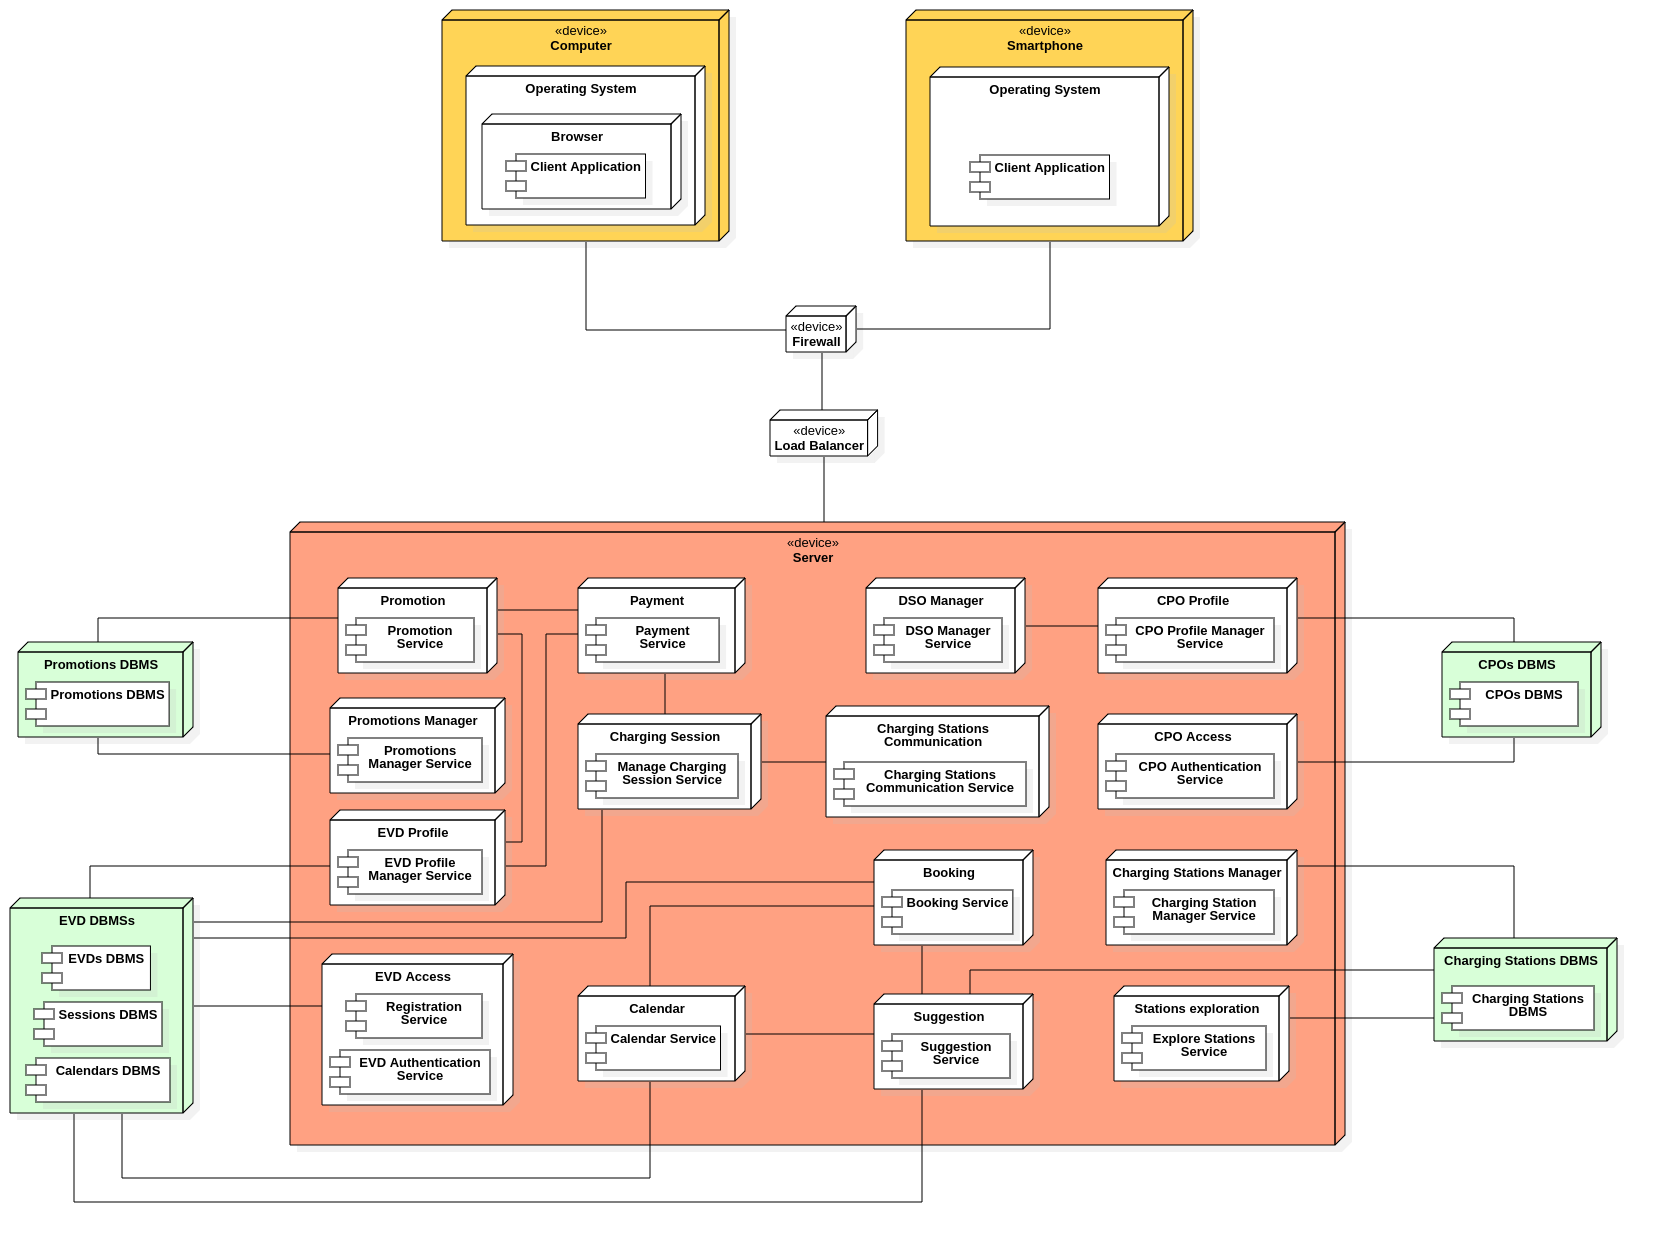
\includegraphics[width=1\linewidth]{DeploymentDiagram/deployment_diagram}
        \caption{Deployment diagram of the eMALL system.}
        \label{fig: depl_diagram}
    \end{center}
\end{figure}

\subsection{Connection to the server}
\label{subsec:connection_to_the_server}%
EVDs and CPOs can access the eMALL system from both PC and smartphones.
In the first case, it is necessary to use a browser to load the system's web page.
In the second case, the client will use the application after downloading it from the smartphone's store (Android or iOS).
When requests are sent to the server, first they pass into the firewall, so to avoid eventual cyberattacks on the system,
then they pass into the load balancer, so to optimize resource usage,
improve performance, and increase the availability of several services.
Requests are now ready to be handled by the eMALL services. \\
It follows the corresponding part from the deployment diagram:
\begin{figure} [H]
    \begin{center}
        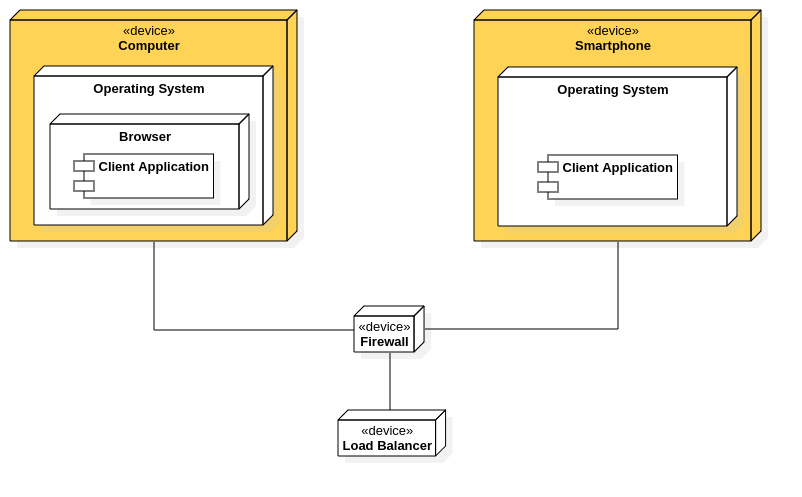
\includegraphics[width=0.7\linewidth]{DeploymentDiagram/connection}
        \caption{Connection to the server diagram.}
        \label{fig: connection}
    \end{center}
\end{figure}

\subsection{Promotions}
\label{subsec:promotions}%
Promotion DBMS is one of the four identified DBMS nodes.
The choice of dividing it from other DBMSs relies on the will to better scale the system.
In this way, it is easier to guarantee the availability of other services that don't work with promotions,
and maintenance sessions are facilitated too.
It has not been grouped with other DBMSs into the same node because Promotions DBMS is also used by CPOs,
so the system needs to guarantee a high level of scalability to assure business functionalities to the companies. \\
It follows the corresponding part from the deployment diagram:
\begin{figure} [H]
    \begin{center}
        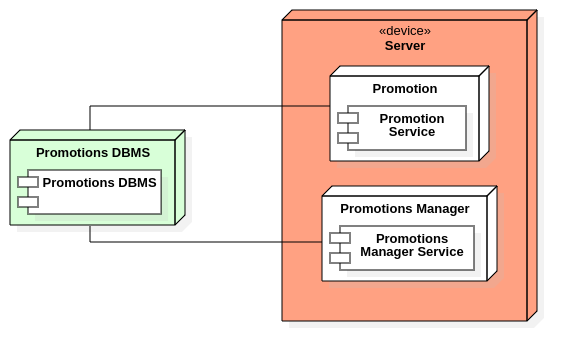
\includegraphics[width=0.6\linewidth]{DeploymentDiagram/promotion}
        \caption{Promotions managing diagram.}
        \label{fig: promotion}
    \end{center}
\end{figure}

\subsection{EVD interactions}
\label{subsec:evd_interactions}%
This section shows how the system communicates with \verb|EVDs DBMS|\@.
We choose to group \verb|EVDs DBMS|, \verb|Sessions DBMS|, and \verb|Calendars DBMS| into the same node because
they all receive requests from the services only in case of interactions with EVDs.
Considering that they don't introduce strict time response requirements,
it was not necessary to insert new physical nodes for the managing of the DBMSs. \\
It follows the corresponding part from the deployment diagram:
\begin{figure} [H]
    \begin{center}
        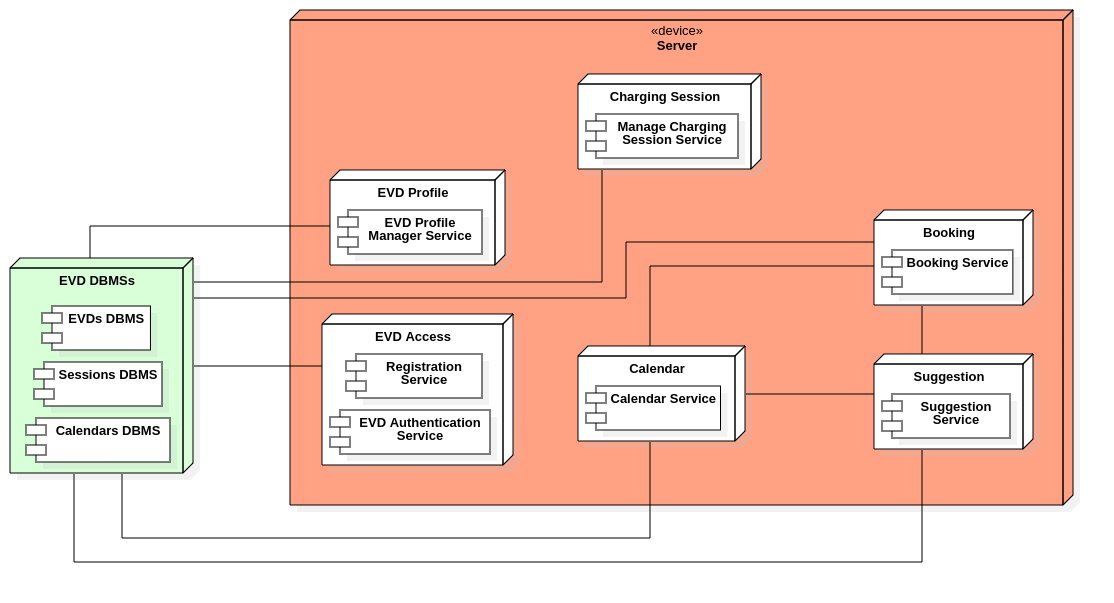
\includegraphics[width=\linewidth]{DeploymentDiagram/EVD_interactions}
        \caption{EVD interactions diagram.}
        \label{fig: evd_interactions}
    \end{center}
\end{figure}

\subsection{CPOs DBMS}
\label{subsec:cpo_dbms}%
The components that communicate with the CPOs DBMS are the Authentication Service and the CPO Profile Manager Service.
When another service needs to get or to update information about a CPO, the request is handled by the CPO Profile node.
The DBMS is used by CPOs, so it is deployed in a single node to better scale the system,
and to guarantee business functionalities to the companies. \\
It follows the corresponding part from the deployment diagram:
\begin{figure} [H]
    \begin{center}
        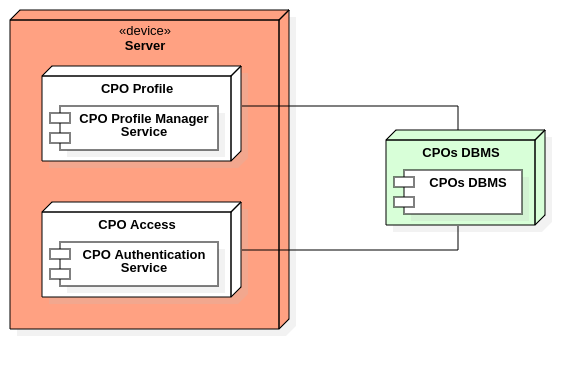
\includegraphics[width=0.6\linewidth]{DeploymentDiagram/CPO_DBMS}
        \caption{CPOs DBMS managing diagram.}
        \label{fig: cpo_dbms}
    \end{center}
\end{figure}

\subsection{Charging stations communication}
\label{subsec:charging_stations_communication}%
Suggestion and Stations exploration nodes read from the DBMS
to get the position of the stations that will be elaborated or shown to the user.
Charging Station Manager Service can also write or update the instances of the DBMS\@.
The DBMS is used by CPOs, so it is deployed in a single node to better scale the system,
and to guarantee business functionalities to the companies. \\
It follows the corresponding part from the deployment diagram:
\begin{figure} [H]
    \begin{center}
        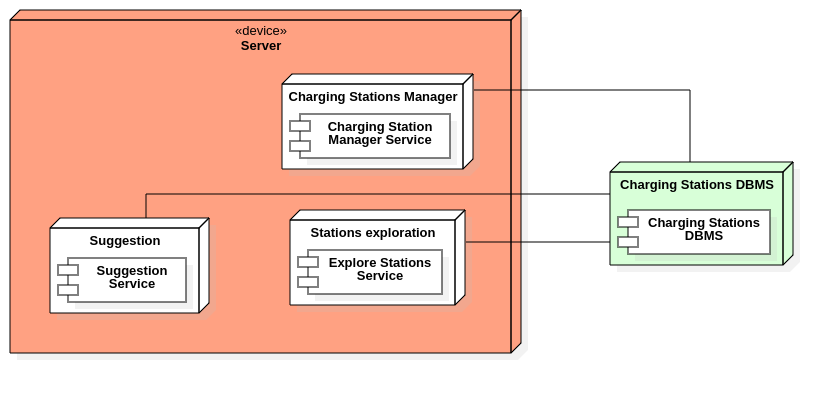
\includegraphics[width=0.85\linewidth]{DeploymentDiagram/charging_stations_communication}
        \caption{Charging stations communication diagram.}
        \label{fig: charing_stations_dbms}
    \end{center}
\end{figure}

\subsection{Services}
\label{subsec:services}%
The section shows all the identified nodes in which services run. \\
Decisions have been made giving particular attention to the concepts of loose coupling and high cohesion.
As explained in Sam Newman's \textit{Building Microservices}, they are defined as follows:
\begin{itemize}
    \item \textbf{Loose coupling.} \textit{When services are loosely coupled, a change to one service should not require a change to another.
    The whole point of a microservice is being able to make a change to one service and deploy it,
        without needing to change any other part of the system.}
    \item \textbf{High Cohesion.} \textit{We want related behavior to sit together, and unrelated behavior to sit elsewhere.
    Making changes in lots of different places is slower, and deploying lots of services at once is risky, both of which we want to avoid.}
\end{itemize}
The following image wants also to highlight the relations between different services, which are direct consequences of the
communication interfaces previously shown in the component diagram.
\begin{figure} [H]
    \begin{center}
        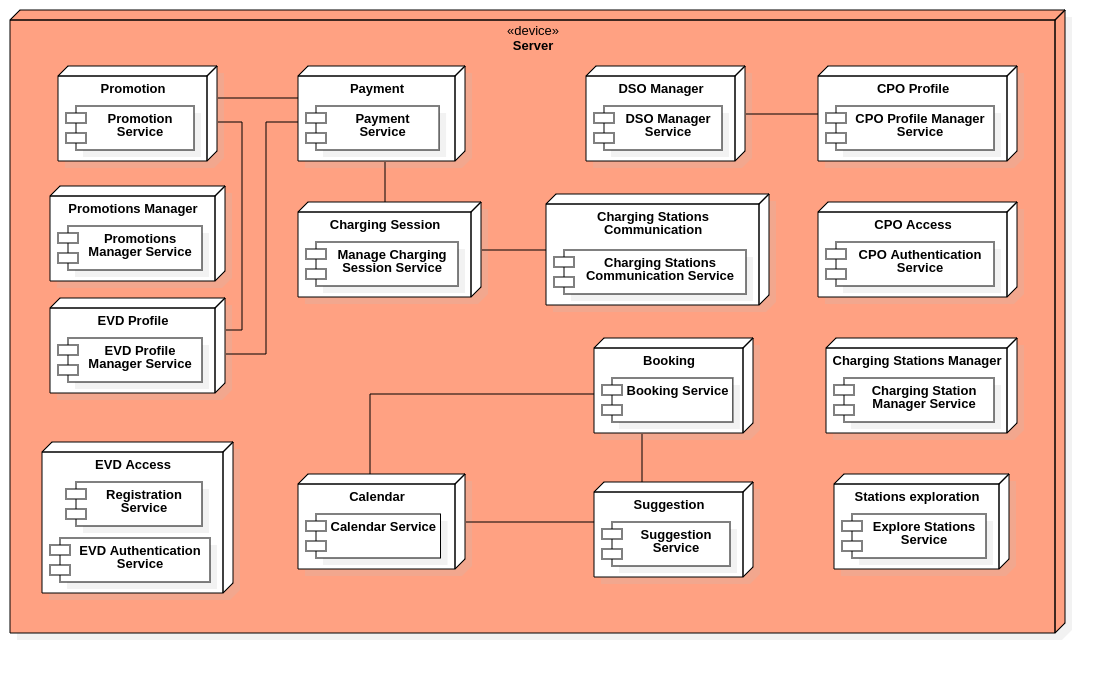
\includegraphics[width=\linewidth]{DeploymentDiagram/server}
        \caption{Server services diagram.}
        \label{fig: services}
    \end{center}
\end{figure}


\section{Runtime View}
\label{sec: runtime_view}%


\section{Component Interfaces}
\label{sec: component_interfaces}%


\section{Selected Architectural Styles and Patterns}
\label{sec: patterns}%


\section{Other Design Decisions}
\label{sec: other_design_decisions}%
